\resizebox{1\columnwidth}{!}{
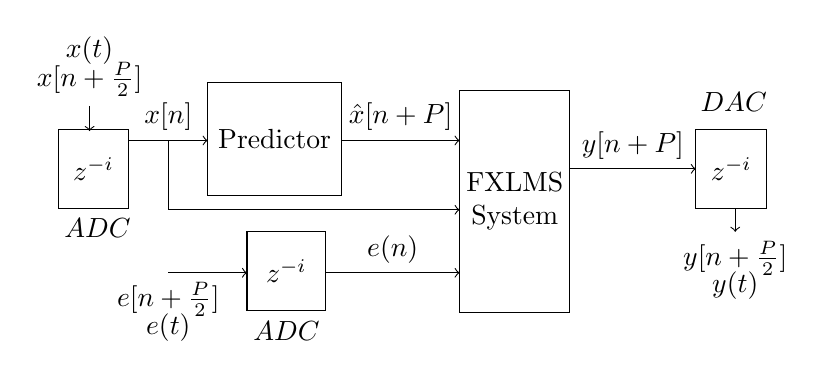
\begin{tikzpicture}
\draw  (-3.7,1.5) rectangle node {$z^{-i}$} (-4.6,0.5);
\draw (-4.1,0) node[above]{$ADC$} ;
\draw (-1.7,-1.3) node[above]{$ADC$} ;
\draw  (-2.7,2.1) rectangle  node[align=center] {Predictor} (-1,0.66) ;

\draw  (0.5,2) rectangle node[text width=1.5cm,align=center] {FXLMS System}(1.9,-0.82);
\draw  (3.5,1.5) rectangle node {$z^{-i}$}(4.4,0.5);
\draw (3.98,1.6) node[above]{$DAC$} ;

\draw [->](-3.7,1.36)  -- (-2.7,1.36);


\draw [->](-1,1.36)  -- node[above]{$\hat{x}[n+P]$}  (0.5,1.36);
\draw [->](1.9,1) -- node[above]{$y[n+P]$} (3.5,1);

\draw [->](-4.2,1.8) node[above]{$x[n+\frac{P}{2}]$} -- (-4.2,1.48);
\draw (-4.2,2.2) node[above]{$x(t)$} ;
\draw [->](4,0.5)-- (4,0.2) node[below]{$y[n+\frac{P}{2}]$} ;
\draw [->](-3.2,1.36) node[above]{$x[n]$} -- (-3.2,0.48) -- (0.5,0.48);
\draw (4,-0.78) node[above]{$y(t)$} ;
\draw  (-1.2,0.2) rectangle node {$z^{-i}$} (-2.2,-0.8);


\draw [->](-1.2,-0.32) -- node[above]{$e(n)$} (0.5,-0.32);
\draw [<-](-2.2,-0.32)-- (-3.2,-0.32) node[below]{$e[n+\frac{P}{2}]$} ;
\draw (-3.2,-1.32) node[above]{$e(t)$} ;
\end{tikzpicture}}